

\chapter{Regression and Classification} 

\section{Basics of Machine Learning}
\subsection{Learning Algorithms}\label{learning-algs}

To understand machine learning, we must begin with the definition of a learning algorithm.

\begin{definition}
A \define{learning algorithm} is a computer program which accomplishes some task (which we will denote $T$) based on some experience ($E$) with respect to some performance measure ($P$), such that performance $P$ increases as we add experience to $E$.
\end{definition}

\begin{remark}
    This is not a true definition of a learning algorithm, but we will understand what is meant by $E, T,$ and $P$ in this section through examples.
\end{remark}

\subsection{Experience}

In a machine learning context, experience is a set of examples that we wish to learn from. Similar to the colloquial use, a learning algorithm 'experiences' these examples and uses them for a variety of tasks, including making predictions or generating new information. 

\begin{definition}
\define{Experience E}  is a dataset $\MX\in\mathbb{R}^{m \times n}$, where each column is called a \define{feature} and each row is called an \define{example}. 
\end{definition}

\begin{example}
A classic example is the Iris dataset. Suppose we have the following measurements for 150 Iris plants.\\

\begin{figure}
\begin{tabular}{p{6cm}c}
   {$\displaystyle 
   \MX = 
   {\renewcommand{\arraystretch}{1.2}
    \begin{bmatrix}
        2.5 & 1.2 & 4.5 & 2.6 \\
        3   & .5 & 3.4  & 4.3 \\
        4.2 & 1.3 & 4.3 & 1.2 \\
        \vdots & \vdots & \vdots & \vdots \\
        3.1 & .7 & 3 & 4.1 \\
        \end{bmatrix}}
    $}
&
$\vcenter{\hbox{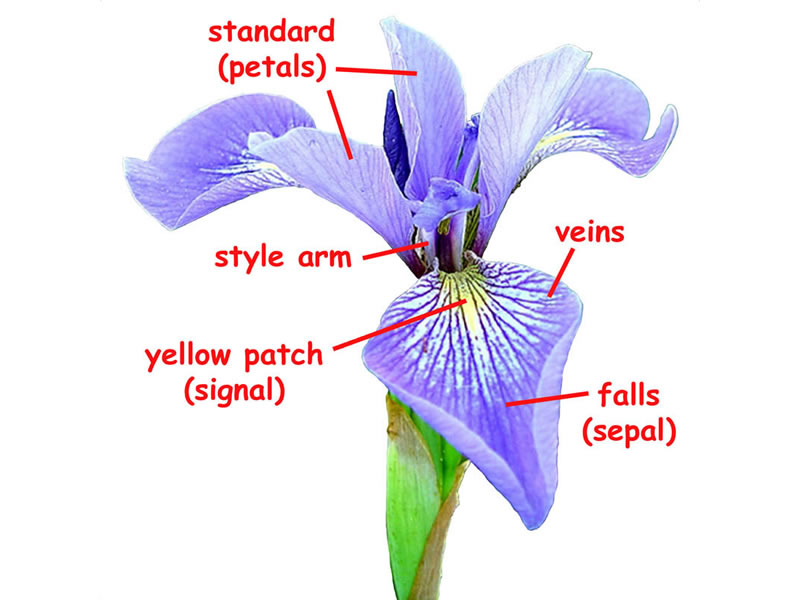
\includegraphics[width=2.5in]{images/Chapter6/iris_diagram_labeled.jpg} }}$
\end{tabular} 
\caption{(Left) Dataset of Iris feature measurements with columns petal length, petal with, sepal length, and sepal width in that order. (Right) Diagram of an Iris with features labeled.}
\end{figure} 

This dataset is our experience. It may also include a vector $\vy$ that catagorizes the plants. For example, we could know that each flower is one of three species, and have the following vector $\vy$: 
$$\MX = 
\begin{bmatrix}
    3 \\
    1 \\
    2 \\
    \vdots \\
    1
    \end{bmatrix}$$

\end{example}

\begin{definition}
A learning algorithm with both $\MX, \vy$ is called \define{supervised}. A learning algorithm with  $\MX$ and no label vector is called \define{unsupervised}. 
\end{definition}
When using an unsupervised algorithm, we determine a probability distribution $p(\vx)$ where $\vx \in \mathbb{R}^n$ corresponds to $x_{i,\ast}$. When using a supervised algorithm, we usually want to determine the probability $p(y|\vx)$. 

\begin{definition}
If $vy$ takes discrete values, we call this a \define{classification} problem. If $vy$ takes continuous values, we call this \define{regression} problem. 
\end{definition}


\subsection{Task}

The next part to understand about learning algorithms is the task $T$. Again, we will improve our understanding through the examples of classification and regression.

The task $T$ of (supervised) classification is generally the following: Given $(\MX, \vy)$ with $y_i \in \{ 1, 2, \ldots, k \}$, produce a function $f: \R^n \to \{ 1, 2, \ldots, k \}$ such that $f(\vx) = y$ performs well as a prediction.

\begin{example}
Suppose $\MX_{i,\ast}$ contains the pixel data of a grayscale image, and $\vy$ has the labels for cats and dogs, say 1 for cats and 2 for dogs arbitrarily. Then one possible task $T$ for a learning algorithm could be to classify a given image $\vx$ as a 1 or 2, or a dog or a cat.
\end{example}

The task $T$ of regression is similar to that of classification: Given $(\MX, \vy)$ with $y_i \in \R$, produce a function $f: \R^n \to \R$ such that $f(\vx) = y$ performs well as a prediction.

\begin{example}
Housing prices are notoriously difficult to predict, but you might want to use data about houses to determine a good price. One way to do this is to collect data on houses and their prices, such as square footage, number of bedrooms, number of bathrooms, and proximity to schools. Each house's data would be kept in $\MX_{i,\ast}$, with the corresponding price in $y_i$. The task $T$ of a learning algorithm with this information could be to predict the price of a house given the data.
\end{example}

There are many other possible examples for regression tasks, such as producing text in Unicode given an image of text, translation between languages, generating new examples from data in experience $E$, filling in missing entries from $\MX$, or removing unwanted noise from $\MX$. In general, defining a task is important because gives meaning to the algorithm. That being said, it is not possible to know how well a given algorithm is doing its task without a performance measure.

\subsection{Performance Measure}

Performance measures $P$ generally depend on the task $T$. For classification algorithms, we often use accuracy, precision, or recall as the performance measure (we will discuss these in future sections). For regression, we often use some sort of average squared error in prediction. This performance is not measured from the experience set $E$, but from a different set of examples, $\MX^{test}$ and the corresponding $\vy^{test}$.

\begin{example}
Let's continue the example for housing prices. Suppose we used a supervised algorithm using experience $E$, say $\MX^{train}$ and $\vy^{train}$. The task $T$ is to generate a function $f : \R^n \to \R$. The performance measure $P$ is the average squared error between $f(\MX^{test})$ and $\vy^{test}$. With this information, we can build a learning algorithm, a computer program, that will attempt to minimize this average squared error.
\end{example}

\section{Linear Regression}

Having covered the basics, we can now discuss how learning algorithms can optimize this performance measure based on the task and experience. For the supervised linear regression model we built in the previous example, we will assume that $y_i$ depends linearly on $\MX_{i,\ast}$. That is, there exist vectors $\vw, \vb$ such that
$$ y_i \approx \MX_{i, \ast} \vw + \vb $$
This is somewhat inconvenient to write with $\vb$ being its own vector, so we introduce the notation
$$\hat{\MX} :=
\begin{bmatrix}
1 & X_{1,1} & X_{1,2} & \cdots & X_{1,n} \\
1 & X_{2,1} & X_{2,2} & \cdots & X_{2,n} \\
\vdots & \vdots & \vdots & \ddots & \vdots \\
1 & X_{m,1} & X_{m,2} & \cdots & X_{m,n} \\
\end{bmatrix}$$
and by optimizing $\vw$ (now an element of $\R^{n+1}$), we get the same result as optimizing $\vw$ and $\vb$ as before. Our optimization will consist of finding the optimal $\vw^\ast$ such that
$$ \frac{1}{m} \sum \limits_{i=1}^m \lVert \hat{\MX}_{i,\ast} \vw - y_i \rVert_2^2 =  \frac{1}{m} \lVert \hat{\MX} \vw - \vy \rVert_2^2$$
is minimized. We will call this our cost function.

\begin{definition}
A \define{cost function} is a function $J : \R^n \to \R$ that takes parameters from experience $E$ and has an argument $\vw$ for which it returns the "cost."
\end{definition}

\begin{note}
$J$ takes on many names, such as cost function, loss function, or error function. The task $T$ is usually related to minimizing $J$, but if we wanted to maximize $J$, we might not call it a cost function, as our intuition tells us that we want to minimize costs. One way to get around this is to minimize the negative of $J$, where $-J$ would be the cost function. This will maximize $J$.
\end{note}

For this particular cost function, we take parameters $\MX$ (changed to $\hat{\MX}$) and $\vy$ from $E$. One solution to finding the optimal $\vw$ to minimize this function is to use gradient descent to approximate $\vw^\ast$.

\begin{proposition}
$J$ is twice-differentiable, convex, has Lipschitz-continuous gradient, has gradient
$$\nabla_{\vw} J(\vw) = \frac{2}{m} (\hat{\MX}^\intercal \hat{\MX} \vw - \hat{\MX} ^\intercal \vy)$$
and has Hessian
$$ H(J)(\vw) = \frac{2}{m} \hat{\MX} ^\intercal \hat{\MX} $$
\begin{proof}
Let $J(\vw)
= \frac{1}{m} (\lVert \hat{\MX} \vw - \vy \rVert_2^2)
= \frac{1}{m} ((\hat{\MX} \vw - \vy)^\intercal (\hat{\MX} \vw - \vy))
= \frac{1}{m} (\vw^\intercal \hat{\MX}^\intercal \hat{\MX} \vw - \vw^\intercal \hat{\MX}^\intercal \vy - \vy^\intercal \hat{\MX} \vw + \vy^\intercal \vy)$. Because this is a real value ($J(\vw) \in \R$), we can rewrite this as
$$ J(\vw) = \frac{1}{m} (\vw^\intercal \hat{\MX}^\intercal \hat{\MX} \vw - 2 \vy^\intercal \hat{\MX} \vw + \vy^\intercal \vy) $$
Using our matrix differentiation rules discussed in Section 2.1, we can find
$$ \nabla_\vw J(\vw) = \frac{\partial}{\partial \vw} J(\vw)^\intercal
= \frac{1}{m}(\vw^\intercal (\hat{\MX} ^\intercal \hat{\MX} + (\hat{\MX} ^\intercal \hat{\MX})^\intercal) - 2 \vy^\intercal \hat{\MX})^\intercal
= \frac{2}{m} (\hat{\MX} ^\intercal \hat{\MX} \vw - \hat{\MX}^\intercal \vy) $$
Now to see this is Lipschitz continuous, let $\vv, \vw \in \R^{n+1}$. Then
$$ \lVert \nabla_\vv J(\vv) - \nabla_\vw J(\vw) \rVert_2
= \frac{2}{m} \lVert (\hat{\MX} ^\intercal \hat{\MX} \vv - \hat{\MX}^\intercal \vy) - (\hat{\MX} ^\intercal \hat{\MX} \vw - \hat{\MX}^\intercal \vy) \rVert_2
= \frac{2}{m} \lVert \hat{\MX} ^\intercal \hat{\MX} (\vv - \vw) \rVert_2$$
$$\leq \frac{2}{m} \lVert \hat{\MX} ^\intercal \hat{\MX} \rVert_2 \lVert \vv - \vw \rVert_2$$
By setting $\Lip = \frac{2}{m} \lVert \hat{\MX} ^\intercal \hat{\MX} \rVert_2$ (a constant), we see the gradient is $\Lip$-Lipschitz continuous. Now we calculate the Hessian, $H(J)(\vw)$ with our matrix differentiation rules again.
$$ H(J)(\vw)
= \frac{\partial^2}{\partial \vw^2} J(\vw)
= \frac{\partial}{\partial \vw} \left( \frac{2}{m} (\hat{\MX} ^\intercal \hat{\MX} \vw - \hat{\MX}^\intercal \vy) \right)
= \frac{2}{m} (\hat{\MX} ^\intercal \hat{\MX})$$
$\hat{\MX} ^\intercal \hat{\MX}$ is positive semidefinite because $\vw^\intercal \hat{\MX} ^\intercal \hat{\MX} \vw = \lVert \hat{\MX} \vw \rVert_2^2 \geq 0$. Because the Hessian is positive semidefinite, we know $J$ is convex. Therefore, we have shown that $J$ is twice-differentiable, convex, has Lipschitz-continuous gradient, has the gradient and Hessian shown above.
\end{proof}
\end{proposition}
From the section on Gradient Descent Convergence, we have the properties to know that gradient descent will converge to the global minimum, $\vw^\ast$, for this particular cost function.

Gradient descent is a computationally expensive algorithm, and depending on the choices of stopping conditions, it may not converge in a reasonable amount of time. Another solution to finding $\vw^\ast$ is to calculate it directly.
\begin{proposition}
If $\hat{\MX}$ has linearly independent columns, and if $J$ has a global minimum, $\vw^\ast$, then $\vw^\ast = (\hat{\MX} ^\intercal \hat{\MX})^{-1} \hat{\MX}^\intercal \vy$.
\begin{proof}
Since $J$ is differentiable, if $\vw^\ast$ is a global minimum, then $\vw^\ast$ is a local minimum, so $\nabla_{\vw^\ast} J(\vw^\ast) = \vzero $. We calculated $\nabla_{\vw^\ast} J(\vw^\ast)$ in the previous problem, so we simply calculate:
$$ \nabla_{\vw^\ast} J(\vw^\ast) = \frac{2}{m} (\hat{\MX} ^\intercal \hat{\MX} \vw^\ast - \hat{\MX}^\intercal \vy) = \vzero$$
$$ \iff \hat{\MX} ^\intercal \hat{\MX} \vw^\ast = \hat{\MX}^\intercal \vy$$
Because $\hat{\MX}$ has linearly independent columns, we know $\hat{\MX} ^\intercal \hat{\MX}$ is positive definite. This means it is invertible, so we have
$$ \vw^\ast = (\hat{\MX} ^\intercal \hat{\MX})^{-1} \hat{\MX}^\intercal \vy $$
Thus we can calculate the minimum, $\vw^\ast$, directly. It can, however, be computationally more expensive to invert matrices, so sometimes it is faster if we simply run gradient descent, which we know will converge.
\end{proof}
\end{proposition}

In the case that $y_i$ is a polynomial function of $\MX_{i,\ast}$, suppose it has maximum total degree $m$. That is, 
$$f(x_1, x_2, \ldots, x_n) = f(\vx) = \sum \limits_{\alpha \in \mathbb{Z}^n} c_\alpha x^\alpha,$$
where $1 \leq \sum \limits_{i=1}^{n} \alpha_i \leq m$. Here is an example of one term of such a polynomial:

\begin{example}
$$ \alpha = (1, 0, 2, 3) \implies x^\alpha = x_1^1 x_2^0 x_3^2 x_4^3 = x_1 x_3^2 x_4^3 $$
The power of $x_i$ is determined by the $i$-th index of $\alpha$.
\end{example}

To solve the case where we assume $y_i$ is a polynomial function of $\MX_{i,\ast}$, we add columns to $\MX$, one for each valid $\alpha \in \mathbb{Z}^n$. Again, we use an example to show what we mean:

\begin{example}
Suppose $\MX = \begin{bmatrix} 1&2\\2&1\\3&4 \end{bmatrix}$. If we assume the maximum total degree is 2, we add columns to $\MX$ and fill in the values:
$$ \phantom{.} \hspace{24mm} \begin{array}{*{5}{c}} x_1 & x_2 & x_1^2 & x_1 x_2 & x_2^2 \end{array} $$
\vspace{-25pt}
$$ \MX = \begin{bmatrix} 1&2\\2&1\\3&4 \end{bmatrix} \to
\begin{bmatrix}
1   &\phantom{..}2  &\phantom{..}1  &\phantom{.}2   &\phantom{.}4\\
2   &\phantom{..}1  &\phantom{..}4  &\phantom{.}2   &\phantom{.}1\\
3   &\phantom{..}4  &\phantom{..}9  &\phantom{.}12  &\phantom{.}16
\end{bmatrix} $$
\end{example}

Doing this sets up a linear relationship between $y_i$ and the new $\MX_{i, \ast}$ because it now contains all of the possible polynomial terms up to degree $m$ of the columns. Then we can form $\hat{\MX}$ as before and solve as in the case of a linear relationship. There is, of course, the problem of picking the "best" maximum total degree $m$, but this problem will be covered in Section 7.2 when we discuss hyperparameters.

\section{Logistic Regression}

Logistic Regression is an instantiation of a Classification Algorithm. The Learning Algorithm is setup as follows
\begin{enumerate}
    \item Experience (E): The dataset $X$ is setup as a $m$ instances, each with $n$ features. More formally, $X \in \R^{m \times n}$. The goal of this algorithm is to predict a binary label for each instance. So, the ground-truth $\vy$ is a vector containing only ones and zeros. So, $\vy \in \{0, 1\}^{m}$. 
    \item Task (T): By observation from the dataset formulation, it becomes clear the goal is to produce a function $f :  \R^{n} \to \{0, 1\}$ learned from each instance $m$. We can then use pass this value through a piece-wise function to assign labels. 
    \item Performance Measure (P): Many choices exist, let's go with accuracy:
    $$\textbf{Acc} = \frac {\#\{i \mid \text{pred}_f(\MX_{i, *}^{\text{(test)}}) = \vy_i^{\text{(test)}}\}}{\# \text{rows} \  \text{in} \ \MX^\text{(test)}}$$
\end{enumerate}

\subsection{One Solution: Logistic Regression}
Now, let's proceed with an illustration of one solution to the desiderata presented above. Here, there are two cases depending on the nature of the data. 
\begin{enumerate}
    \item Case 1: If we expect $y = 1$ examples are reliably separated from $y = 0$ by a hyperplane in $\R^n$.
    
    \begin{center}
    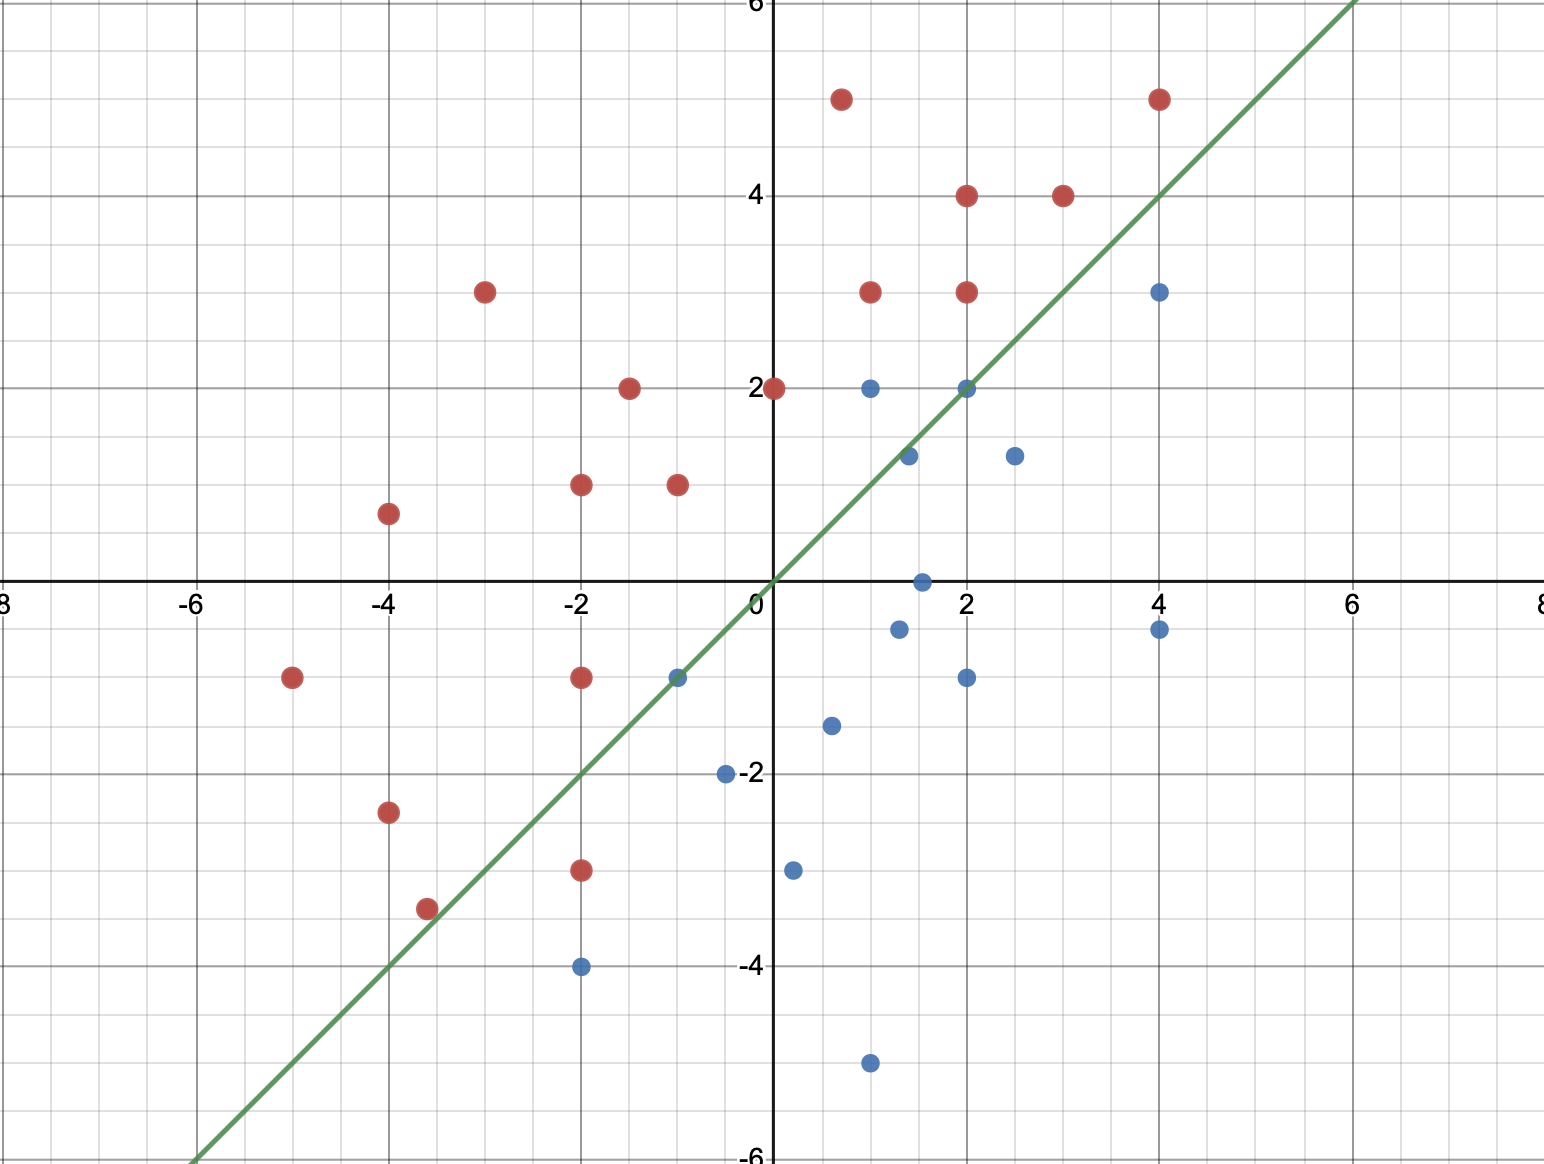
\includegraphics[width=3.5in]{images/Chapter6/logreg_ex.png}
    \end{center}
    
    Goal: Find $\vw \in \R^{n}$ and $\vb \in \R$ such that the hyperplane $\overrightarrow{\vw}^T \overrightarrow{\MX} + \vb = 0$ \footnote{Notice that $\overrightarrow{\vw}$ is a normal vector} separates the $1$'s from $0$'s "reliably". \footnote{There is no concrete definition of a reliable. In this context, we are referring to a dataset which logistic regression would be able to do well on.}
    
    The next question that arises is how to use the optimization machinery previously discussed to learn $\overrightarrow{\vw}$ and $\vb$. Toward this, we need to define a cost function $J(\overrightarrow{\vw}, \vb)$ such that minimizing this objective, maximizes our Performance Measure (Accuracy).
    
    \subsubsection{Observations about current setup}
    The key observation to be made is that $\overrightarrow{\vw} \overrightarrow{\vx} + \vb \in \R$. So, $\overrightarrow{\vw}^T \overrightarrow{\vx} + \vb << 0$ suggests that the model strongly predicts a $0$ or $\overrightarrow{\vw}^T \overrightarrow{\vx} + \vb >> 0$ suggests that the model strongly predicts a $1$. However, the issue here is that we have a prediction \footnote{Such an unnormalized probability distribution is sometimes called an 'energy'. This 'energy'-based formulation of Deep Learning allows for a method to rewrite the optimization function of several algorithms such as Variational Autoencoders and certain Self-Supervised Learning algorithms as an energy function which can then be optimized using your favorite gradient-based optimizer.} in $\R$  and not in $[0, 1]$. So, to proceed forward we need to find a 'normalization' function.
    
    \subsubsection{Desiderata for the Normalization function}
    We want our normalization function $g: \R \to [0, 1]$ to satisfy the following properties:
    $$\lim_{z \to \infty} g(z) = 1$$
    $$\lim_{z \to -\infty} g(z) = 0$$
    $$g(0) = \frac{1}{2}$$ 
    Using a function which satisfies the above properties, we are now able to assign labels through the following piece-wise function:
    $${pred}_f(x) = \twopartdef{1}{x > 0.5}{0}{x \leq 0.5}$$
    
    \subsubsection{The Sigmoid Function}
    Define $g: \R \to [0, 1]$ as:
    $$g(x) = \frac{1}{1 + e^{-x}}$$
    
    \begin{center}
    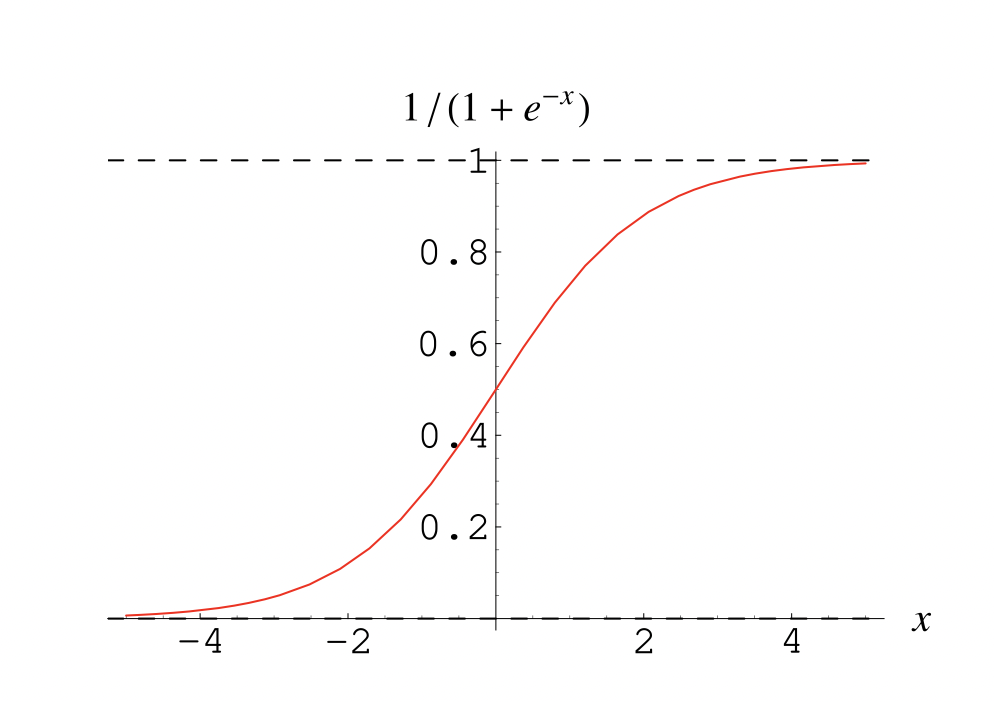
\includegraphics[width=4in]{images/Chapter6/sigmoid.png}
    \end{center}
    \begin{proposition}
    \begin{enumerate}
        \item The Sigmoid Function satisfies all the outlined desiderata of a normalization function.
        \item $g'(x) = g(x)(1 - g(x))$
    \end{enumerate}
    \end{proposition}
    
    \begin{proof}
    This is left as an exercise to the reader.
    \end{proof}
    
    \subsubsection{Designing the Cost Function $J(\overrightarrow{\vw}, \vb)$}
    For sake of notational brevity, we use the $\hat{\MX}$ notation from previous sections. This allows the inference function to be rewritten as $\hat{\MX}\vv$ instead of $\overrightarrow{\vw}^T \overrightarrow{\MX} + \vb$.
    

    We have to have a cost function which encourages two cases: $$g(\overrightarrow{\vx}^T\overrightarrow{\vv}) >> 0 \  {if} \  y = 1$$
    $$g(\overrightarrow{\vx}^T\overrightarrow{\vv}) << 1 \  {if} \  y = 0$$
    
    Intuitively, we want to penalize the inverse behavior. If the ground-truth is $1$ we want to penalize on learning values which would lead to a $0$ prediction and vice-versa.
    
    Another way to express this is to penalize with the following scheme:
    $$\overrightarrow{\vv} \ {if} \  y = 1 \ \& -\log(g(\overrightarrow{\vx}^T\overrightarrow{\vv})) >>> 0$$
    $$\overrightarrow{\vv} \ {if} \  y = 0 \ \& -\log(1 - g(\overrightarrow{\vx}^T\overrightarrow{\vv})) >>> 0$$ 
    
    The final bit of insight we can exploit is in the nature of the problem. In all cases, $\vy$ is either $0$ or $1$. So, we can use this fact to serve as a gate between the two cases of the cost function. Hence, we can penalize $\vv$ if $-\vy \log(g(\overrightarrow{\vx}^T\overrightarrow{\vv})) - (1 - \vy) \log(1 - g(\overrightarrow{\vx}^T\overrightarrow{\vv}))$ is large. 
    
    Finally, all we are left to do is accumulating this cost function over the whole train dataset.
    
    \begin{definition}
    Given $\MX^{{(train)}}, \vy^{{(train)}}$, define $log: \R^m \rightarrow \R^m$ $$\log(x_1, ... , x_m) = (\log(x_1), ... , \log(x_m))$$ and $G: \R^m \rightarrow \R^m$ $$G(x_1, ... , x_m) = (g(x_1), ... , g(x_m))$$
    $$J(\vv) = \frac{1}{m} \sum_{i = 1}^{m} - (1 - \vy_i)\log(1 - g(\overrightarrow{\vx_{i,*}}^T\overrightarrow{\vv})) -\vy \log(g(\overrightarrow{\vx_i}^T\overrightarrow{\vv}))$$
       which can be rewritten in the more conventient notation of matrix multiplication: 
    $$J(\vv) = \frac{1}{m}[-(\overrightarrow{1} - \overrightarrow{\vy})^T \log(\overrightarrow{1} - \overrightarrow{G}(\hat{\MX}\overrightarrow{\vv})) - \overrightarrow{\vy}^T \log(G(\hat{\MX}\overrightarrow{\vv})]$$
    
    and find $\vv^* = argmin (J(\vv))$ using some form of gradient descent.
    
    \end{definition}
    
    \begin{proposition}
        $$\nabla{v}J(\vv) = \frac{1}{m}(G(\hat{\MX}\overrightarrow{\vv}) - \overrightarrow{\vy})^T\hat{\MX}$$
        $$H(J)(\vv) = \frac{1}{m}\hat{\MX}^TD(\vv)\hat{\MX}$$
        $$D(\vv) = diag(G'(\hat{\MX}\overrightarrow{\vv}))$$
        $$G'(x_1, ... , x_m) = (g'(x_1), ... , g'(x_m))$$
        J is twice differentiable convex, and has Lipschitz continuous gradient.
 
    Therefore gradient descent reliably finds the global minimum (if it exists).
    \end{proposition}

    \begin{proof}
    This proof is left as an exercise to the reader.
    \end{proof}    
    
    \item Case 2: A non-linear "Decision Boundary"
    
    In this case, one may find this nonlinear decision boundary by modifying x by adding new columns corresponding to polygons or other functions of current columns. \footnote{Playing around with the dataset in this way is called \textit{feature engineering}. Feature Engineering can often end up being more of an art than a science as a whole lot of intuition is required in order to guess what features the model would need to then linearly separate the modified feature space.}
\end{enumerate}

\section{Exercises}

\begin{enumerate}
    \item We discussed the tasks of classification and regression algorithms. Provide possible tasks for the following experience sets, and state whether the learning algorithm would be classification or regression.
    \begin{enumerate}
        \item $\MX$ with red, green, and blue pixel values as the columns and $\vy$ with numbers corresponding to colors (for example, 0 for red, 1 for blue, 2 for green, 3 for yellow)
        \item $\MX$ with data that seems to cluster around different areas in $\R^n$.
        \item $\MX$ with data about three notes in one bar of a 4/4 time signature and $\vy$ with the fourth note.
    \end{enumerate}
    \item Suppose we have $\MX, \vy$:
    $$ \MX = \begin{bmatrix}
    5 & 3 & 1\\
    4 & 4 & 2\\
    1 & 2 & 1
    \end{bmatrix}, \vy =
    \begin{bmatrix}
    31\\
    34\\
    30
    \end{bmatrix} $$
    and a cost function:
    $$ J(\vw) = \frac{1}{3} \lVert \hat{\MX} \vw - \vy \rVert_2^2$$
    Given $\vv = \begin{bmatrix}
    1\\
    0.6\\
    7\\
    3
    \end{bmatrix}$, calculate $J(\vv)$.
    \item Define $\MX$:
    $$\MX =
    \begin{bmatrix}
    1&2&3\\
    2&4&2\\
    3&3&5
    \end{bmatrix}$$
    Assume there is a polynomial relationship between the associated $\vy$ and $\MX$, and that the maximum total degree of said polynomial is 2. Set up the new $\MX$ such that the relationship between some $y_i$ and $\MX_{i,\ast}$ is linear but represents the polynomial combinations of the columns of the current $\MX$.
\end{enumerate}

\section{Solutions to Exercises}
\begin{enumerate}
    \item Here are some possible solutions:
    \begin{enumerate}
        \item A classification algorithm that would take in $\vx \in \R^3$ and output a number corresponding to the predicted color.
        \item Suppose the data in $\MX$ clusters around $k$ different points. Then a regression algorithm with this dataset might first determine what the $k$ different center points in $\R^n$ then, given $\vx \in \R^n$, classify which of the $k$ center points it clusters around.
        \item A regression algorithm that, given $\vx \in \R^3$ which represents the first three notes, will predict the fourth note in the bar.
    \end{enumerate}
    \item First we must construct $\hat{\MX}$, then we can calculate $J(\vv)$.
    $$ J(\vv) = \frac{1}{3} \left\lVert
    \begin{bmatrix}
    1 & 5 & 3 & 1\\
    1 & 4 & 4 & 2\\
    1 & 1 & 2 & 1
    \end{bmatrix}
    \begin{bmatrix}
    1\\
    0.6\\
    7\\
    3
    \end{bmatrix}
    -
    \begin{bmatrix}
    31\\
    34\\
    30
    \end{bmatrix}
    \right\rVert_2^2$$
    $$
    =
    \frac{1}{3} \left\lVert
    \begin{bmatrix}
    31\\34.4\\28.6
    \end{bmatrix}
    -
    \begin{bmatrix}
    31\\34\\30
    \end{bmatrix}\right\rVert_2^2
    =
    \frac{1}{3} \left\lVert
    \begin{bmatrix}
    0\\0.4\\-1.4
    \end{bmatrix} \right\rVert_2^2 = \frac{1}{3} (2.12) \approx 0.70667$$
    \item Our new $\MX$ is:
    $$\phantom{\MX=}\setlength\arraycolsep{8pt}
    \begin{array}{*{9}{c}} x_1 & x_2 & x_3 & \hspace{-4pt}x_1x_2 & \hspace{-6pt}x_1x_3 & \hspace{-5pt}x_2x_3 & \hspace{-1pt}x_1^2 & \hspace{3pt}x_2^2 & \hspace{3pt}x_3^2 \end{array} $$
    \vspace{-15pt}
    $$
    \MX =
    \setlength\arraycolsep{10pt}
    \begin{bmatrix}
    1   &2  &3  &2  &3  &6  &1  &4  &9\\
    2   &4  &2  &8  &4  &8  &4  &16 &4\\
    3   &3  &5  &9  &15 &15 &9  &9  &25
    \end{bmatrix} $$
\end{enumerate}